\documentclass[conference]{IEEEtran}
\IEEEoverridecommandlockouts
% The preceding line is only needed to identify funding in the first footnote. If that is unneeded, please comment it out.
\usepackage{cite}
\usepackage{amsmath,amssymb,amsfonts}
\usepackage{algorithmic}
\usepackage{graphicx}
\usepackage{textcomp}
\usepackage{xcolor}
\usepackage{subcaption}
\def\BibTeX{{\rm B\kern-.05em{\sc i\kern-.025em b}\kern-.08em
    T\kern-.1667em\lower.7ex\hbox{E}\kern-.125emX}}
\begin{document}

\title{Efficient Neuromorphic Data Processing: A Unified Framework for Pipeline Optimization and Lightweight Preprocessing*\\
{\footnotesize \textsuperscript{*}Note: Sub-titles are not captured in Xplore and
should not be used}
\thanks{Identify applicable funding agency here. If none, delete this.}
}

\author{\IEEEauthorblockN{1\textsuperscript{st} Given Name Surname}
\IEEEauthorblockA{\textit{dept. name of organization (of Aff.)} \\
\textit{name of organization (of Aff.)}\\
City, Country \\
email address or ORCID}
\and
\IEEEauthorblockN{2\textsuperscript{nd} Given Name Surname}
\IEEEauthorblockA{\textit{dept. name of organization (of Aff.)} \\
\textit{name of organization (of Aff.)}\\
City, Country \\
email address or ORCID}
\and
\IEEEauthorblockN{3\textsuperscript{rd} Given Name Surname}
\IEEEauthorblockA{\textit{dept. name of organization (of Aff.)} \\
\textit{name of organization (of Aff.)}\\
City, Country \\
email address or ORCID}
\and
\IEEEauthorblockN{4\textsuperscript{th} Given Name Surname}
\IEEEauthorblockA{\textit{dept. name of organization (of Aff.)} \\
\textit{name of organization (of Aff.)}\\
City, Country \\
email address or ORCID}
\and
\IEEEauthorblockN{5\textsuperscript{th} Given Name Surname}
\IEEEauthorblockA{\textit{dept. name of organization (of Aff.)} \\
\textit{name of organization (of Aff.)}\\
City, Country \\
email address or ORCID}
\and
\IEEEauthorblockN{6\textsuperscript{th} Given Name Surname}
\IEEEauthorblockA{\textit{dept. name of organization (of Aff.)} \\
\textit{name of organization (of Aff.)}\\
City, Country \\
email address or ORCID}
}

\maketitle

\begin{abstract}
To address the computational efficiency bottleneck in real-time processing of neuromorphic data (e.g., DVS128 Gesture), 
this paper proposes an end-to-end acceleration solution that integrates data pipeline optimization and lightweight preprocessing. 
At the system level, the use of \texttt{num\_workers} for parallel loading and \texttt{prefetch\_factor} for prefetching significantly enhances the throughput of the data pipeline. 
At the algorithmic level, a dynamic time window event frame aggregation method based on spatiotemporal sparsity is introduced, along with a low-computation pulse noise filtering module leveraging local spatiotemporal correlations. 
Additionally, structured model pruning is employed to reduce redundant connections and lower computational overhead. Experimental results demonstrate that on an NVIDIA 4070 GPU, the inference speed on the test set is doubled, 
while achieving classification accuracies of 92.36\% (test set) and 98.97\% (training set). 
This work combines data pipeline optimization with lightweight preprocessing, providing a high real-time solution for neuromorphic data processing in edge computing scenarios, with significant practical engineering value.
\end{abstract}

\begin{IEEEkeywords}
Neuromorphic Computing, Data Pipeline Optimization, Pulse Noise Filtering
\end{IEEEkeywords}

\section{Introduction}
Spiking Neural Networks(SNN),which are regarded as the third generation of neural network models,offer a more biologically plausible simulation of neural dynamic by incorporating not only neuronal and synaptic states but also temporal information into their computational framework.\cite{b3,10.5555}Unlike traditional artificial neural networks (ANNs),which relay on continuous-valued activations,SNNs process information through discrete spike events,letting them to capture the temporal dependencies inherent in biological systems.This temporal sensivity,combined with energy-efficient computation,allows SNNs to become as a promising alternative for modeling complex cognitive tasks with potentially superior performance and lower power consumption.\cite{roy2019towards}

Neuromorphic data, characterized by its event-driven nature and sparse sensory representation, has emerged as a compelling paradigm across various real-time application domains, including gesture recognition, object tracking, and autonomous navigation. Neuromorphic data, characterized by its event-driven nature and sparse sensory representation, has emerged as a compelling paradigm across various real-time application domains, including gesture recognition, object tracking, and autonomous navigation.However, the efficient processing of such data remains a significant challenge, particularly in edge computing scenarios where computational resources are limited. A critical bottleneck lies in the substantial latency introduced by data loading and preprocessing. Traditional approaches to address this issue often focus on either algorithmic optimizations or hardware acceleration in isolation, failing to fully exploit the synergistic potential of a unified framework.\cite{ding2024}

This paper proposes a novel solution that seamlessly integrates data pipeline optimization with lightweight preprocessing techniques to achieve end-to-end acceleration. At the system level, we leverage parallel loading and prefetching mechanisms to maximize data throughput. On the algorithmic front, we introduce a computationally efficient pulse noise filtering module based on local spatiotemporal correlations.This module enhances the robustness of our model against noise while preserving critical temporal dynamics. Additionally, we incorporate a self-attention mechanism to augment the model's understanding of feature channel interdependencies, thereby improving its representational capacity.\cite{hu2019} To further enhance computational efficiency, we employ structured model pruning,which systematically reduces redundant connections.\cite{han2015}

Our contributions are threefold:

(1)we compared the effects on accuracy and training speed when setting different frame numbers in the ddateset.

(2)we proposed a lightweight preprocessing method that combines pulse noise filtering and self-attention mechanisms based on the network proposed by WeiFang\cite{fang2021}to enhance the model's robustness and representational capacity.Meanwhile we conducted experiments on the DVS-Gesture dataset and achieved experimental results.

(3)we introduced structured model pruning to reduce redundant connections, thereby improving computational efficiency.


\section{Related Work}
\subsection{Spiking Neural Networks}
Spiking Neural Networks(SNNs) mimics the pulse emission characteristics of biological neurons, drives computing with discrete events, and has significant advantages in energy-sensitive scenarios (such as edge devices).\cite{roy2019towards} A major research focus in the field of SNNs is the conversion from artificial neural networks(ANNs) to SNNs\cite{rueckauer2017conversion},which is dedicated to addressing the challenges of accuracy degradation and training instability during the conversion process.\cite{han2020rmp} Zhang et al. (2025) proposed a method called STNN-SNN, a Spatial-Temporal Attention Aggregator SNN framework,which can dynamically attend to and capture dependencies between spatial and temporal domains.\cite{zhang2025}

\subsection{Spatial-Temporal-Polarity Coherence Filtering}
In event-based neuromorphic data processing, spatio-temporal polarity coherent filtering is an effective denoising processing method. Unlike conventional frame-based filtering, this method leverages the unique characteristics of event streams, where each event is defined by its spatial coordinates, timestamp, and polarity. Spatio-temporal polarity coherent filtering has been widely applied in event-based neuromorphic vision tasks. Sironi et al.(2018) used polarity and spatial-temporal neighborhood statistical characteristics to robustly classify events.\cite{8578284} 

\subsection{Attention Mechanism of SNNs}
Attention mechanism has attracted considerable attention since its inception and has been widely used in various neural network architectures.Xue et al. (2024) introduced Gated Attention Coding (GAC)\cite{qiu2024}, a plug-and-play module that encodes inputs into powerful representations.Yu et al. (2024) proposed a Frequency-based Spatial-Temporal Attention(FSTA) model to enhance feature learning in SNNs.\cite{yu2025}  Shen et al.(2024) innovatively implemented an attention mechanism in SNNs called Temporal Interaction Module (TIM),which was designed to augment the temporal data processing abilities within SNN architectures.\cite{shen2024}


\section{Methodology}
in this section, we first introduce the fundamental computational units of SNNs,namely the most widely used spiking neuron:the Leaky Integrate-and-Fire (LIF) neuron\cite{10.5555/2728336.2728412}.Then,we discussed the polarity coherence filtering method used for dataset denoising. At last, we present the model improved with Squeeze-and-Excitation Block (SEBlock).\cite{hu2019}
\subsection{LIF neuron}
An LIF neuron is depicted by the following equations:
\begin{equation}
\tau \frac{dV(t)}{dt} = -\left(V(t) - V_{\text{reset}}\right) + I(t)
\end{equation}
where $V(t)$ denotes the membrance potential of neuron at time $t$,$I(t)$ represents the input to neuron at time $t$, $V_{\text{reset}}$ is the reset potential, and $\tau$ is the time constant of the neuron. When the membrane potential $V(t)$ goes beyond the certain threshold $V_{\text{thresh}}$, the neuron will emit a spike and reset its membrane potential to $V_{\text{reset}}$. The output spike can be defined as:
\begin{equation}
S(t) = \begin{cases}
1, & \text{if } V(t) \geq V_{\text{thresh}} \\
0, & \text{otherwise}
\end{cases}
\end{equation}
where $S(t)$ is the output spike at time $t$. The LIF neuron model captures the essential dynamics of biological neurons, which includes the integration of inputs over time and the generation of discrete spikes based on membrane potential thresholds.
\subsection{Spatio-temporal polarity coherence filtering: formula analysis}
Given an event stream $\mathcal{E} = \{e_i\}_{i=1}^N$, where each event $e_i = (t_i, x_i, y_i, p_i)$ consists of timestamp $t_i$, spatial coordinates $(x_i, y_i)$, and polarity $p_i \in \{0, 1\}$, the processing consists of two main steps: polarity-consistent filtering and temporal frame integration.

\subsubsection{Polarity-Consistent Spatio-Temporal Filtering}

For each event $e_i$, define its feature vector as:
\[
\mathbf{f}_i = \left( \left\lfloor \frac{t_i}{\Delta t} \right\rfloor, x_i, y_i \right)
\]
where $\Delta t$ is the time window (e.g., 1000).

Construct a $k$-d tree using all $\mathbf{f}_i$ and, for each event, find its neighbors within radius $r$:
\[
\mathcal{N}_i = \left\{ j \mid \|\mathbf{f}_j - \mathbf{f}_i\|_2 \leq r \right\}
\]

An event $e_i$ is retained if the number of neighbors with the same polarity exceeds a threshold $\theta$:
\[
\sum_{j \in \mathcal{N}_i} \mathbb{I}(p_j = p_i) > \theta
\]
where $\mathbb{I}(\cdot)$ is the indicator function.

\subsubsection{Temporal Frame Integration (16 Frames Example)}

Let the filtered events be $\{e_k\}_{k=1}^{N'}$ with timestamps $t_k$. Define $t_{\text{start}} = t_1$, $t_{\text{end}} = t_{N'}$, and total duration $T = t_{\text{end}} - t_{\text{start}}$.

Set the base frame width and remainder as:
\[
d = \left\lfloor \frac{T}{16} \right\rfloor, \quad r = T \bmod 16
\]

For frame $i$ ($i = 0, 1, \ldots, 15$), the time interval is:
\begin{align}
t_{\text{low}}^{(i)} &= t_{\text{start}} + i \cdot d + \min(i, r) \\
t_{\text{high}}^{(i)} &= t_{\text{low}}^{(i)} + d + \delta_i
\end{align}
where
\begin{equation}
\delta_i =
\begin{cases}
1, & i < r \\
0, & i \geq r
\end{cases}
\end{equation}

Each frame $F_i$ is constructed by accumulating events in $[t_{\text{low}}^{(i)}, t_{\text{high}}^{(i)})$:
\[
F_i(c, x, y) = \sum_{k \in \mathcal{S}_i} \mathbb{I}(x_k = x, y_k = y, p_k = c)
\]
where $\mathcal{S}_i = \{k \mid t_{\text{low}}^{(i)} \leq t_k < t_{\text{high}}^{(i)}\}$ and $c \in \{0, 1\}$ denotes the polarity channel.

The final output is a tensor of shape $16 \times 2 \times H \times W$.

\subsection{The model improved with Squeeze-and-Excitation Block (SEBlock)}
when the filtering process for the dataset is completed, we can use the processed dataset to train the model. In this paper we proposed a model based on the WeiFang's model\cite{fang2021} and improved it with Squeeze-and-Excitation Block (SEBlock)\cite{hu2019},alongside we conducted various experiments on this model and performed detailed comparisons.The model architecture is shown in Fig \ref{fig:model} and more Specific details will be presented in the following sections.
\begin{figure}[htbp]
    \centering
    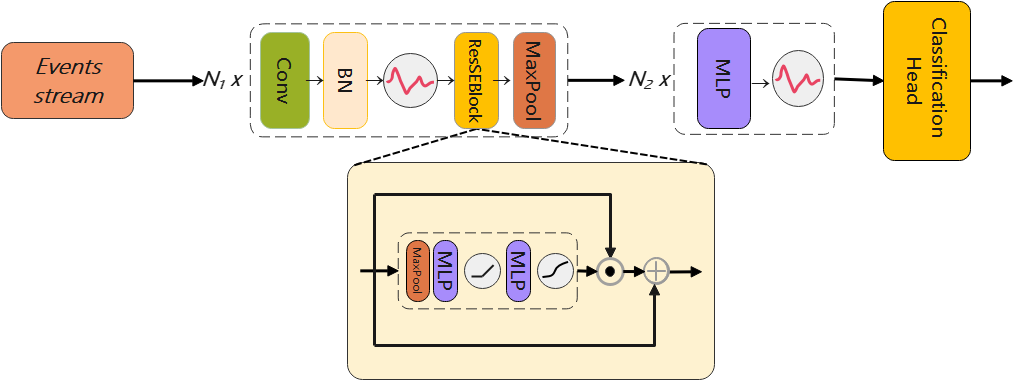
\includegraphics[width=0.45\textwidth]{figure/model.png}
    \caption{The Model Architecture with Squeeze-and-Excitation Block (SEBlock)}
    \label{fig:model}
\end{figure}






\section{Experiments}
\subsection{Experimental Setup}
\textbf{Dataset Description} In this experiment, we utilize the DVS Gesture dataset, a publicly available dataset for gesture recognition based on Dynamic Vision Sensor (DVS). 
The dataset comprises 1,342 samples, each corresponding to one of 11 distinct gesture categories.
Each gesture is performed multiple times by approximately 29 different subjects. 
Each sample is stored in the form of an event stream. 
The dataset also provides training and test set splits, facilitating model evaluation on real-world event data.
The data was collected under varying lighting and motion conditions to enhance diversity.

\textbf{Evaluation Metrics} To comprehensively evaluate model performance, we employ five key metrics: 
(1) Training speed (samples/sec), measuring computational efficiency by tracking processed samples per second during training; 
(2) Training accuracy (\%), monitoring the model's learning progress by calculating correct predictions on training data; 
(3) Test accuracy (\%), the primary classification metric evaluated on held-out test samples;
(4) Training loss, recorded as an observational metric to analyze model behavior during training; 
(5) Test loss, evaluating generalization capability on held-out data. 

All experiments were conducted on a single NVIDIA RTX 4070 GPU with a batch size of 16, using the Adam optimizer, 
Automatic Mixed Precision (AMP) for faster computation, and the CuPy library for GPU-accelerated array operations. 
This multi-faceted evaluation captures both computational efficiency (training speed) and model effectiveness (accuracy/loss), 
while the training loss serves purely as a diagnostic indicator rather than a control signal.

\subsection{Impact of Frame Count on Model Performance}
When processing DVS Gesture data, it is often necessary to convert the raw event stream into some form of image representation (e.g., event frames, accumulated frames, or time surfaces) so that it can be input into a convolutional neural network (CNN) for classification or other tasks. In this process, frame number is a key parameter, which indicates how many time windows the entire event stream should be divided into. Within each window, an "event frame" is generated as an input feature.

In this experiment, we process the DVS Gesture dataset on different frame numbers, as shown in Fig \ref{fig:dvs_gesture_frame_num}. Each row represents the processed dataset with different frame numbers, from top to bottom the number of frames is 2, 4, 8, and 16. And each column represents a different category, from left to right, which is guitar, right hand wave, forearm roll forward, left hand wave, right hand counter clockwise, right hand clockwise, left hand counter clockwise, left hand clockwise, clap, drums and others.
\begin{figure}
    \centering
    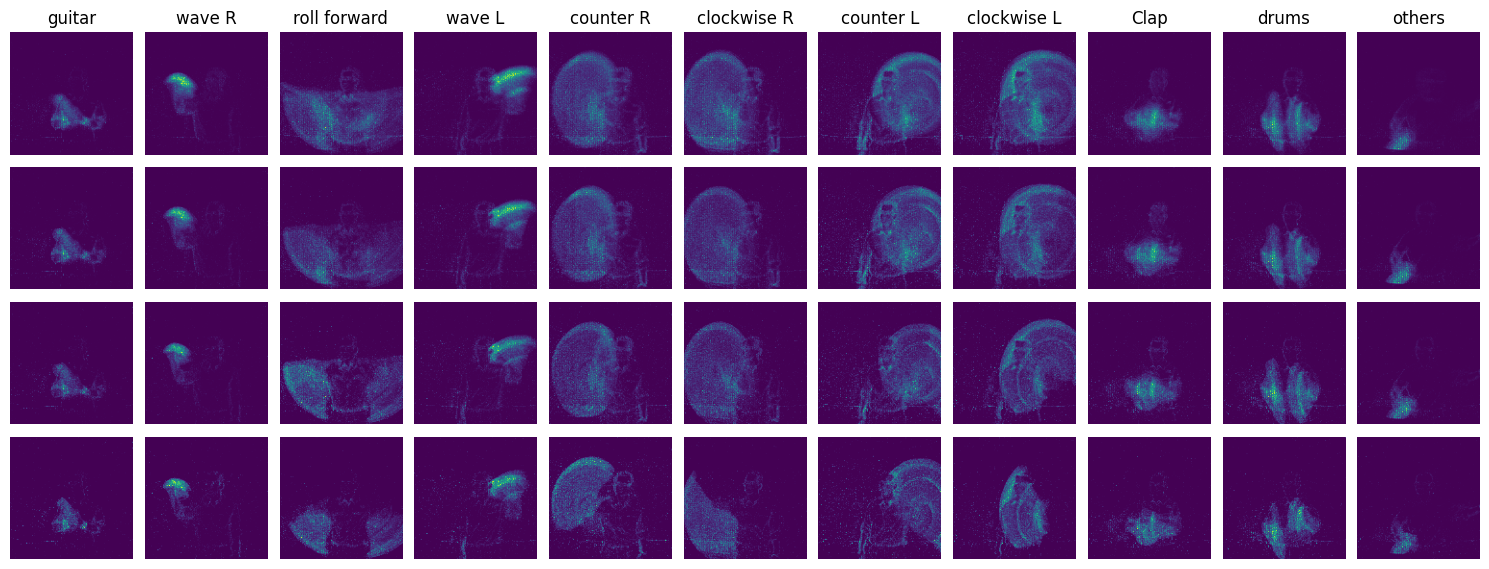
\includegraphics[width=0.45\textwidth]{figure/dataset.png}
    \caption{DVS Gesture Dataset in Different Frame Numbers}
    \label{fig:dvs_gesture_frame_num}
\end{figure}

Through the sample of dataset, we can see that for most categories there is only a change in brightness caused by the difference of frame number, but for certain categories, such as the counter clockwise and clockwise rotation of the left and right hands, it is difficult to distinguish the corresponding images in the dataset with a small number of frames.

To detect the influence of frame number on the model training, we use the DVS Gesture dataset processed with different frame numbers to train the basic model and compare the performance of the model. The corresponding training results are shown in Fig\ref{fig:main_figure}.
\begin{figure}[htbp]
    \centering
    \begin{subfigure}[b]{0.24\textwidth}
        \centering
        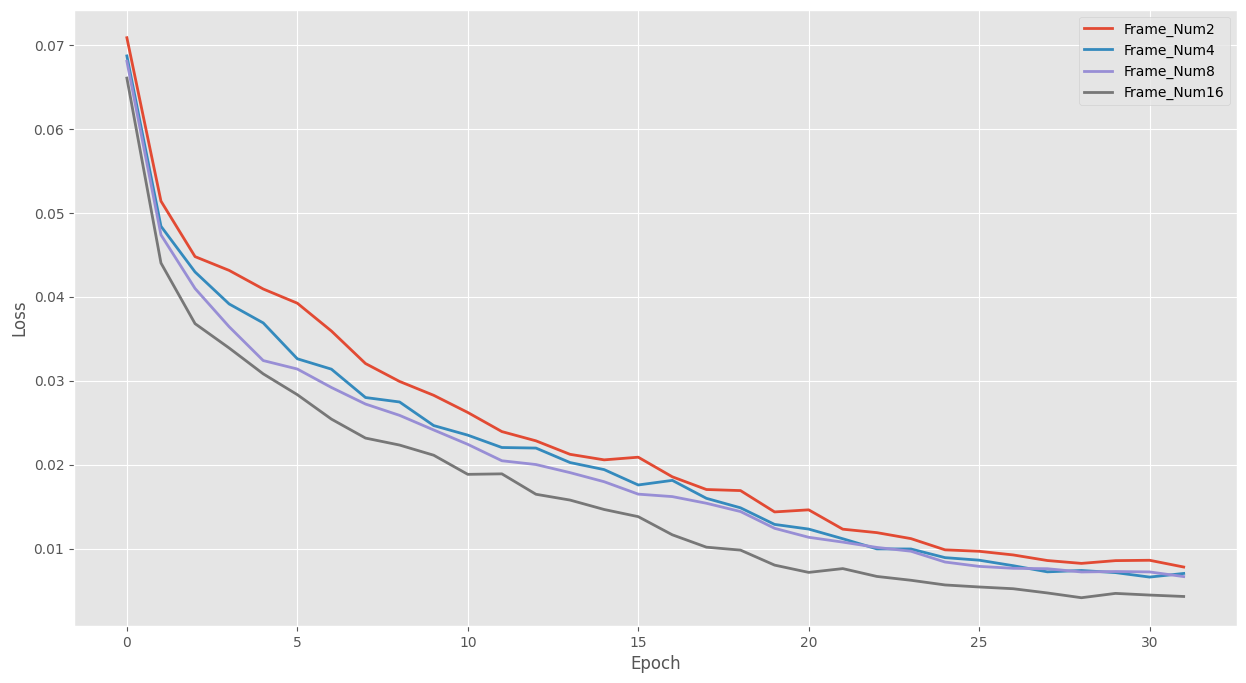
\includegraphics[width=\textwidth]{figure/Train_loss.png}
        \caption{Train Loss Curve}
        \label{fig:sub1}
    \end{subfigure}
    \begin{subfigure}[b]{0.24\textwidth}
        \centering
        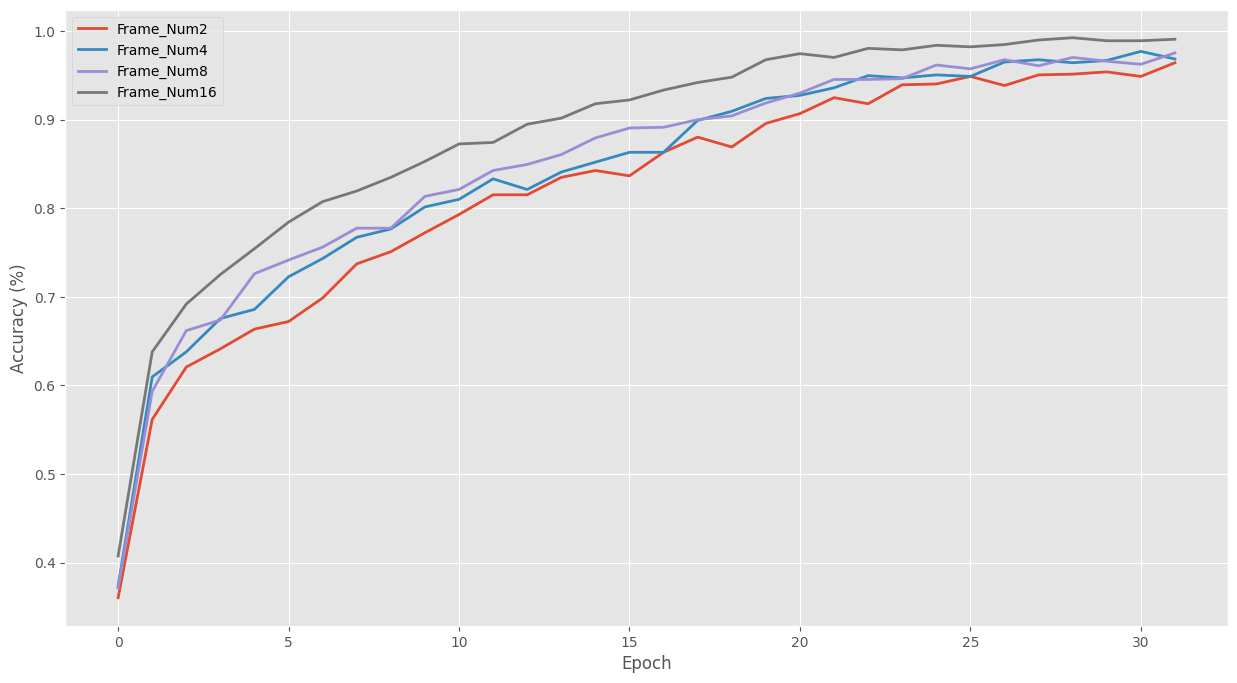
\includegraphics[width=\textwidth]{figure/Train_acc.png}
        \caption{Train Accuracy Curve}
        \label{fig:sub2}
    \end{subfigure}

    \vspace{0.01em} % Adjust vertical space between rows

    \begin{subfigure}[b]{0.24\textwidth}
        \centering
        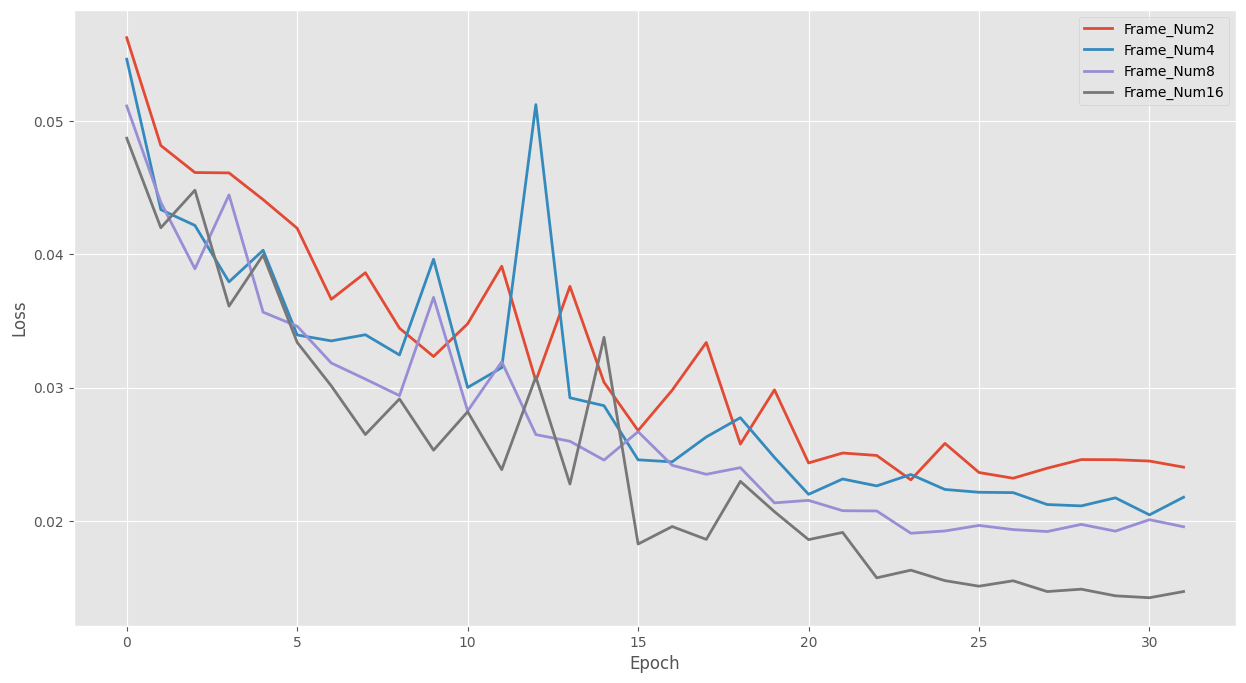
\includegraphics[width=\textwidth]{figure/Test_loss.png}
        \caption{Test Loss Curve}
        \label{fig:sub3}
    \end{subfigure}
    \begin{subfigure}[b]{0.24\textwidth}
        \centering
        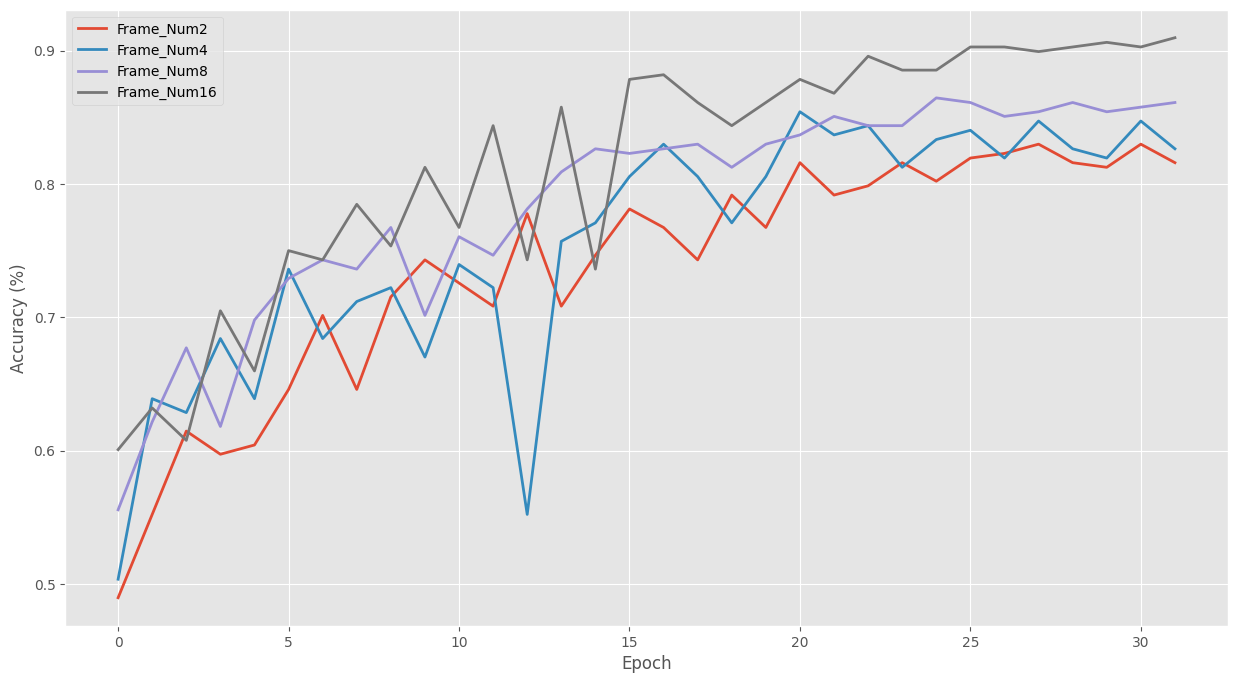
\includegraphics[width=\textwidth]{figure/Test_acc.png}
        \caption{Test Accuracy Curve}
        \label{fig:sub4}
    \end{subfigure}
    \caption{Base Model Performance Under Varying Frame Numbers}
    \label{fig:main_figure}
\end{figure}

The results show that the model with more frames can achieve higher accuracy.The Fig\ref{fig:main_figure} demonstrate that the frame partitioning strategy exhibits negligible impact on both model loss and accuracy during the initial 10 training epochs. However, subsequent training reveals a significant performance divergence - higher frame counts consistently yield superior results, with the baseline model achieving lower loss values and higher accuracy when processing certain movement sampled frames. This phenomenon can be attributed to the increased information density afforded by finer temporal segmentation, which enables more comprehensive feature extraction throughout the network's deeper layers.

In addition to loss and accuracy, training speed is also an important metric for evaluating model performance. The Fig\ref{fig:speed-accuracy} below illustrates the relationship between Average training speed and Maximum test accuracy during model training across different frame numbers.
\begin{figure}
    \centering
    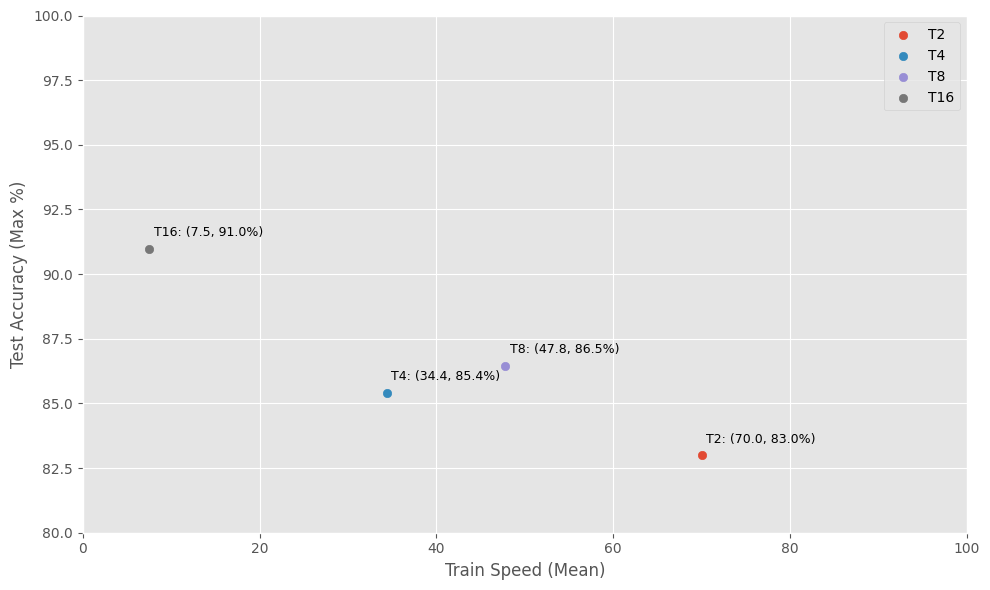
\includegraphics[width=0.45\textwidth]{figure/Accuracy_speed.png}
    \caption{Speed-Accuracy Plot}
    \label{fig:speed-accuracy}
\end{figure}

As shown in Fig\ref{fig:speed-accuracy}, reducing the number of frames per event significantly accelerates the training speed. However, fewer frames lead to a certain degree of information loss, which consequently reduces the accuracy. In this experiment, the highest accuracy of 91.0\% is achieved when each event is divided into 16 frames, while the training speed is the slowest at 7.5. Conversely, when each event is divided into 2 frames, the accuracy drops to its lowest at 83.0\%, but the training speed increases nearly tenfold compared to the slowest speed.

\subsection{Impact of Denoising on Model Efficacy}
To further enhance the model's training performance, we performed denoising on the dataset based on setting the number of frames for event segmentation to 16, aiming to achieve superior training outcomes.We applied the spatio-temporal polarity coherent filtering, as introduced in the Methodology chapter, to process the dataset. 
\begin{figure}[htbp]
    \centering
    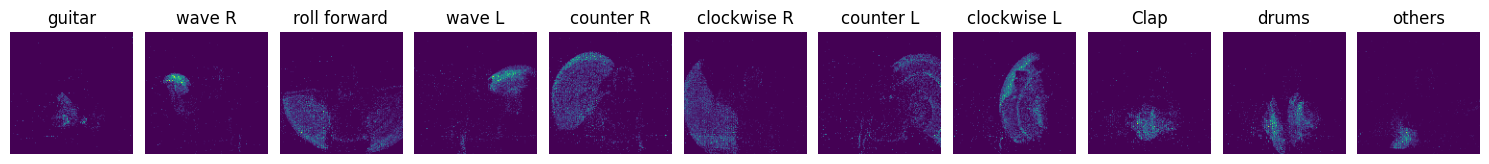
\includegraphics[width=0.45\textwidth]{figure/denoise.png}
    \caption{Denoised Dataset}
    \label{fig:denoise}
\end{figure}

The frame of each category from the processed dataset are illustrated in Fig\ref{fig:denoise}. The denoised images exhibit a high level of clarity and smoothness, with minimal visual artifacts. Essential details, such as edges and textures, are well-preserved, ensuring the integrity of the original data. 
The dataset presents a clean and visually consistent representation, characterized by a uniform and noise-free appearance. The overall visual quality of the denoised images is both natural and interpretable, making them suitable for subsequent analysis.

To further optimize based on the results of the previous experiment, we similarly segmented each event stream in the denoised dataset into 16 frames and trained the baseline model for 32 epochs to compare the training performance. The transformations of key parameters during the training process are shown in Fig\ref{fig:performance-denoise}.
\begin{figure}[htbp]
    \centering
    \begin{subfigure}[b]{0.24\textwidth}
        \centering
        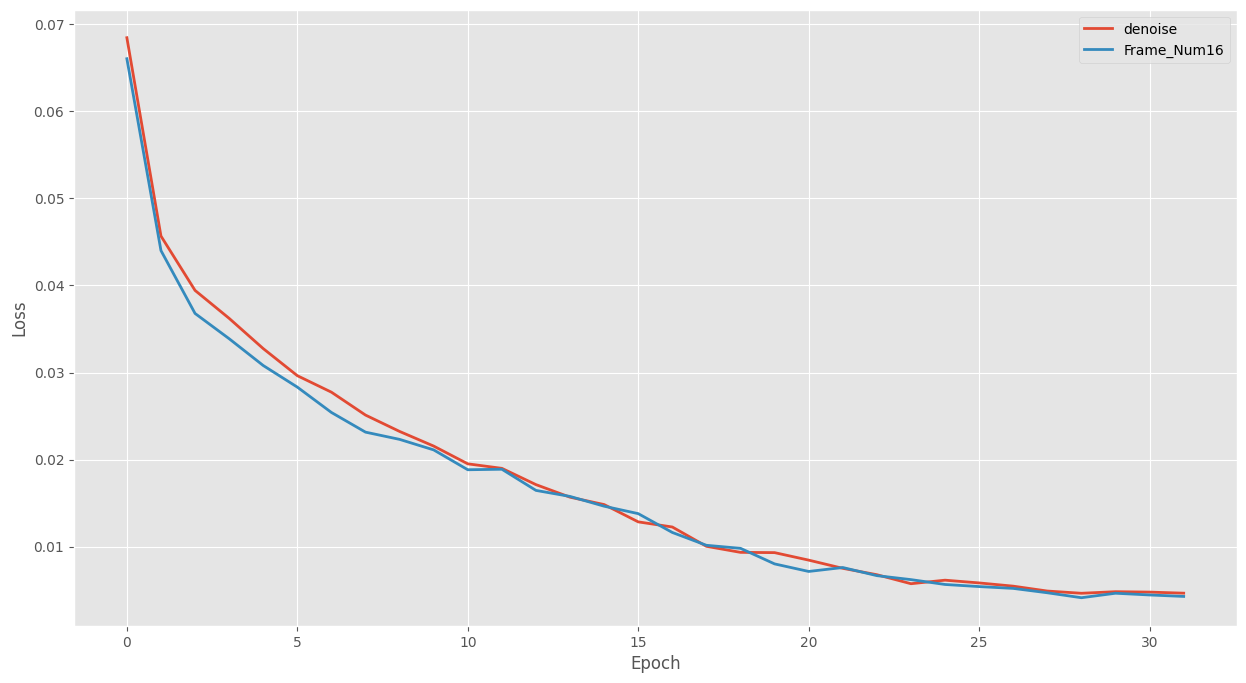
\includegraphics[width=\textwidth]{figure/denoise_train_loss.png}
        \caption{Train Loss Curve}
        \label{fig:sub1-d}
    \end{subfigure}
    \begin{subfigure}[b]{0.24\textwidth}
        \centering
        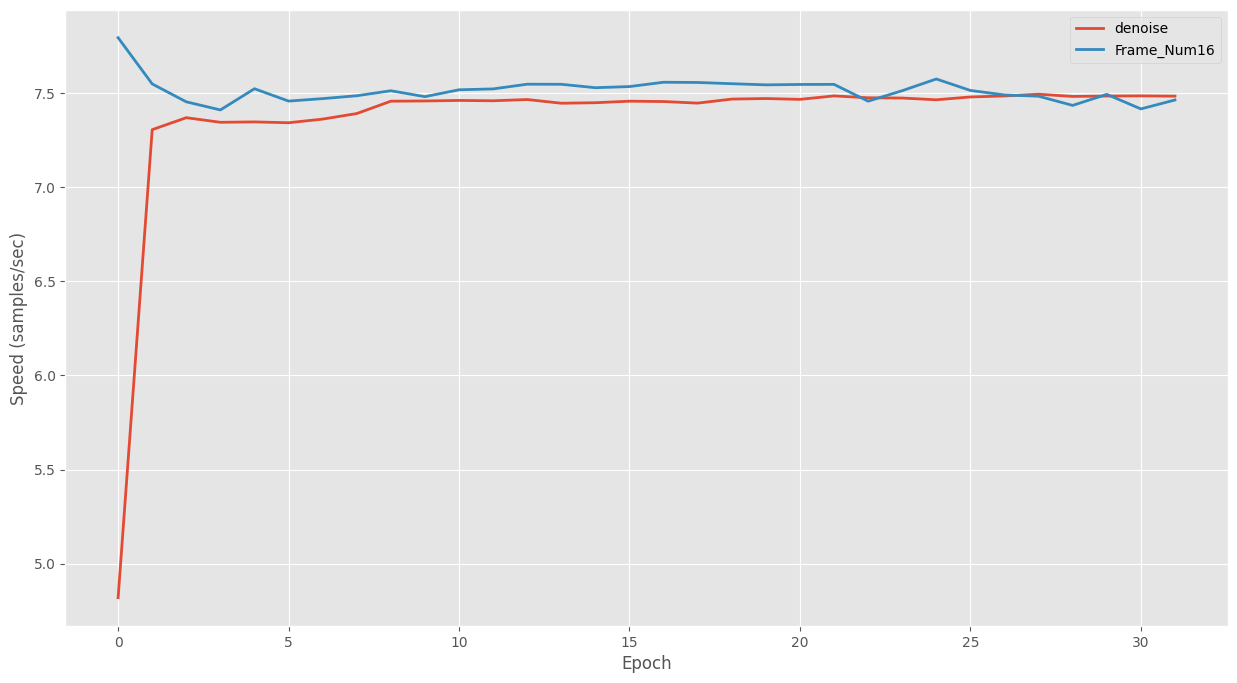
\includegraphics[width=\textwidth]{figure/denoise_train_speed.png}
        \caption{Train Speed Curve}
        \label{fig:sub2-d}
    \end{subfigure}

    \vspace{0.01em} % Adjust vertical space between rows

    \begin{subfigure}[b]{0.24\textwidth}
        \centering
        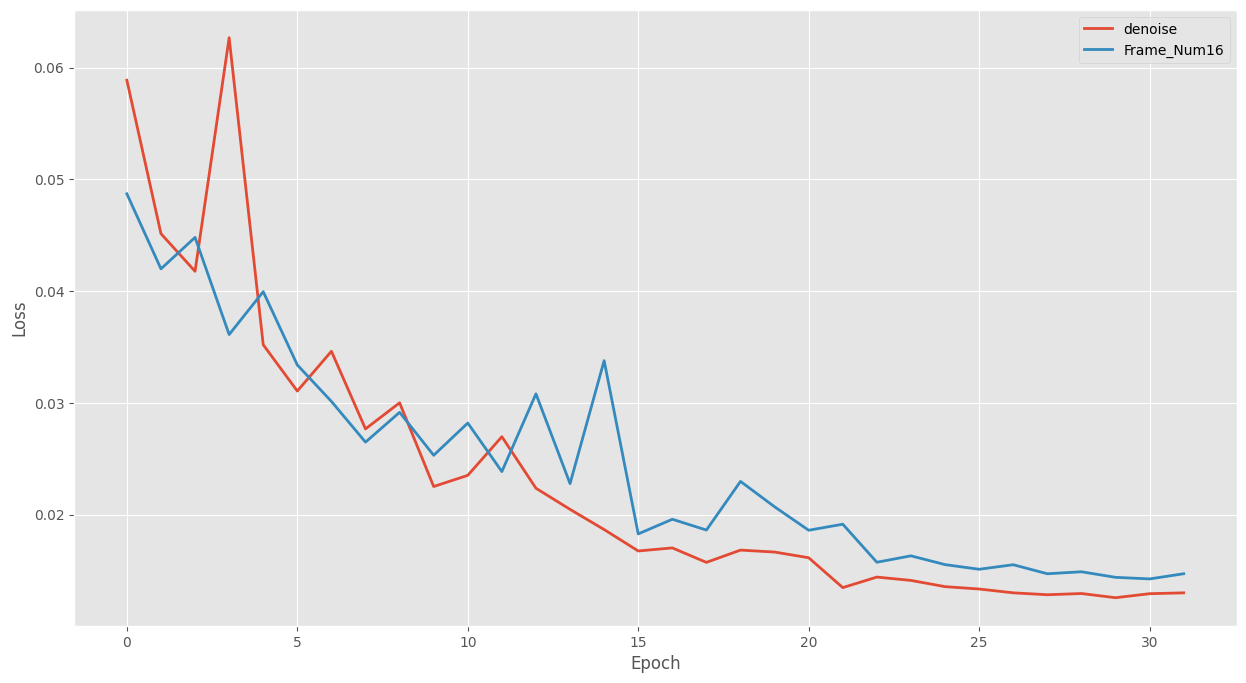
\includegraphics[width=\textwidth]{figure/denoise_test_loss.png}
        \caption{Test Loss Curve}
        \label{fig:sub3-d}
    \end{subfigure}
    \begin{subfigure}[b]{0.24\textwidth}
        \centering
        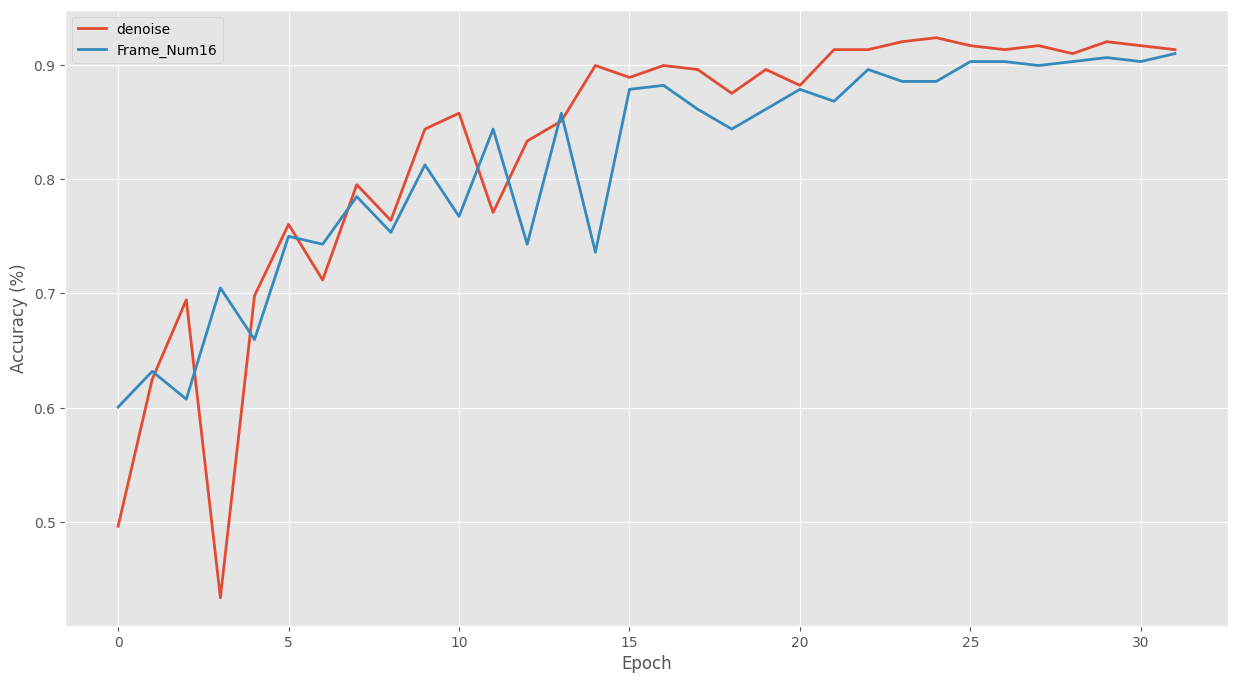
\includegraphics[width=\textwidth]{figure/denoise_test_acc.png}
        \caption{Test Accuracy Curve}
        \label{fig:sub4-d}
    \end{subfigure}
    \caption{Model Performance on Original and Denoised Data}
    \label{fig:performance-denoise}
\end{figure}

By analyzing Fig\ref{fig:sub1-d} and Fig\ref{fig:sub2-d}, which respectively depict the training loss and training speed of basic model on both the original dataset and the denoised dataset, it can be observed that except for the slower training speed of the base model in the first epoch on the denoised dataset compared to the original dataset, the performance of the two datasets during the training process is similar in all other cases. 

The model's test accuracy exhibited a fluctuating upward trend on both the original and denoised datasets. The original dataset achieved its peak accuracy of 91\% at epoch 22, while the denoised dataset reached its maximum accuracy of 92.4\% at epoch 25. Analysis of the loss and accuracy curves during testing revealed that both datasets demonstrated comparable performance within the first 10 epochs. However, in subsequent epochs, the denoised dataset consistently maintained approximately 0.002 lower test loss and nearly 1.4\% higher accuracy compared to the original dataset. This suggests that the denoising operation yields measurable improvements in model training performance.

In summary, the experimental results demonstrate that the denoised dataset outperforms the original dataset during the testing phase, consistently achieving lower test loss and higher accuracy. This superior performance aligns with expectations, as the enhanced data quality resulting from the denoising process contributes to improved model generalization and predictive capability. While both datasets exhibited similar training dynamics beyond the initial epoch, the denoised dataset's advantage in testing metrics underscores the importance of data preprocessing in optimizing model performance.

\subsection{Assessing Model Performance with Attention Mechanism}
In the previous experiment, the denoised dataset demonstrated measurable improvements in the training performance of the baseline model. Building upon these findings, the current experiment incorporates the denoised dataset while introducing an attention mechanism to the original model architecture, followed by a comparative analysis of model performance.

Fig\ref{fig:SE} presents a comparative analysis of training parameter dynamics in both the baseline model and the attention-augmented architecture.
\begin{figure}[htbp]
    \centering
    \begin{subfigure}[b]{0.24\textwidth}
        \centering
        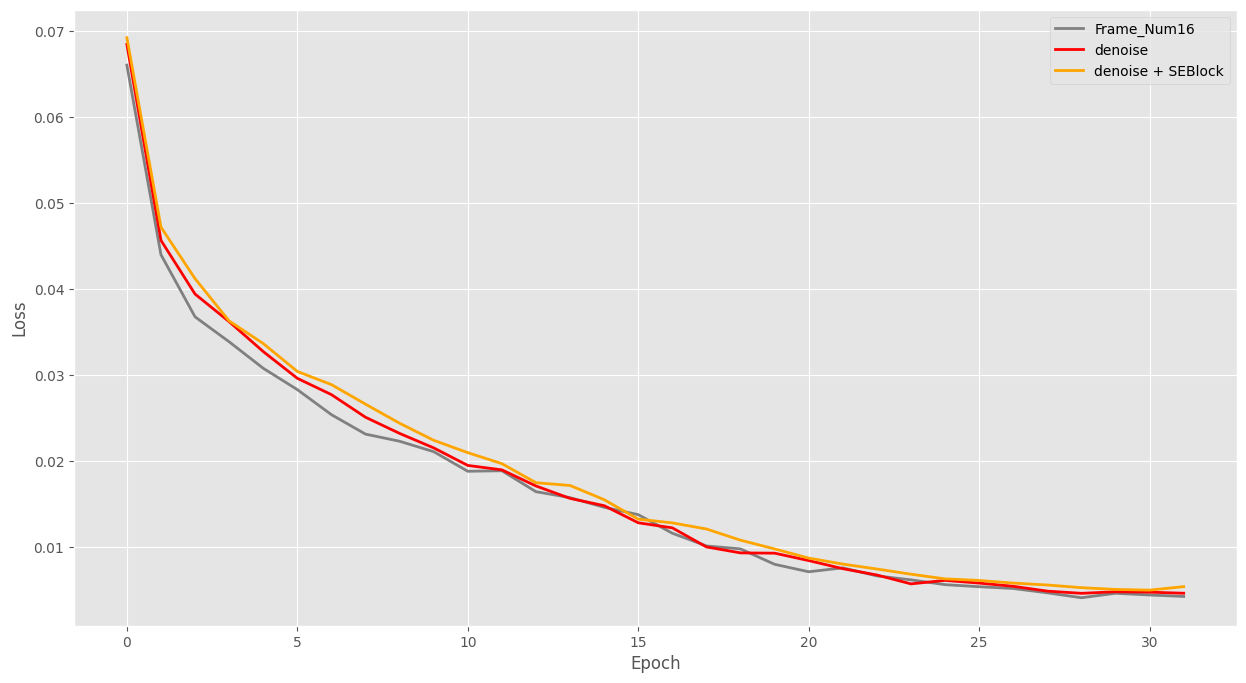
\includegraphics[width=\textwidth]{figure/SE_train_loss.png}
        \caption{Train Loss Curve}
        \label{fig:sub1-SE}
    \end{subfigure}
    \begin{subfigure}[b]{0.24\textwidth}
        \centering
        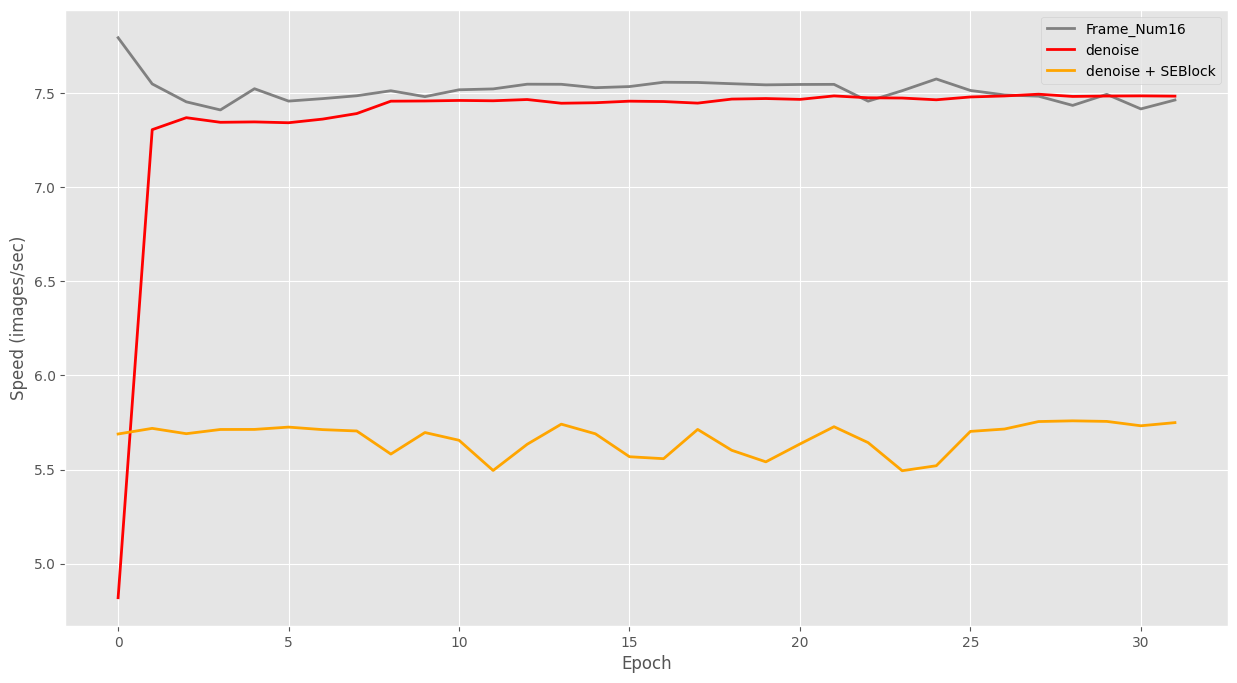
\includegraphics[width=\textwidth]{figure/SE_train_speed.png}
        \caption{Train Speed Curve}
        \label{fig:sub2-SE}
    \end{subfigure}

    \vspace{0.01em} % Adjust vertical space between rows

    \begin{subfigure}[b]{0.24\textwidth}
        \centering
        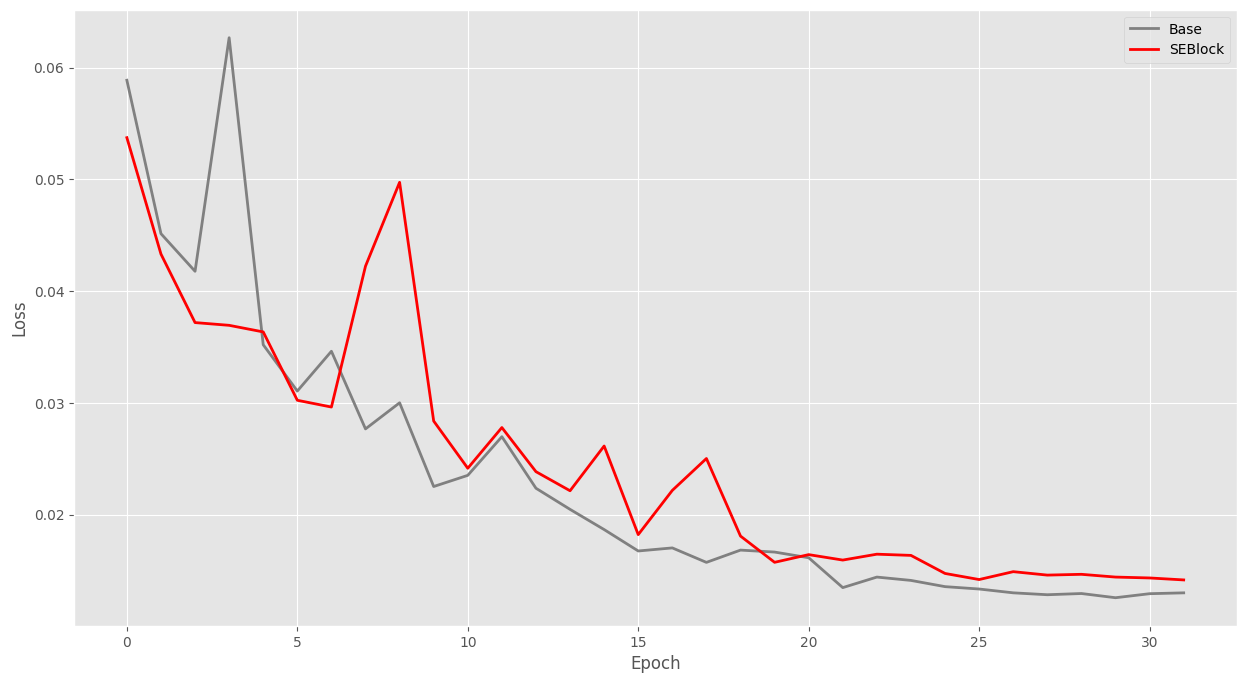
\includegraphics[width=\textwidth]{figure/SE_test_loss.png}
        \caption{Test Loss Curve}
        \label{fig:sub3-SE}
    \end{subfigure}
    \begin{subfigure}[b]{0.24\textwidth}
        \centering
        \includegraphics[width=\textwidth]{figure/SE_test_acc.png}
        \caption{Test Accuracy Curve}
        \label{fig:sub4-SE}
    \end{subfigure}
    \caption{Basa Model and Attention Model Performance on Denoised Dataset}
    \label{fig:SE}
\end{figure}

The Fig\ref{fig:sub1-SE} and Fig\ref{fig:sub2-SE} presents a comparative analysis of the training processes between the SEBlock-integrated model and the baseline model on the denoised dataset. The Fig\ref{fig:sub1-SE} illustrates the loss variation during the training process for both models. The results demonstrate nearly identical loss trajectories between the two architectures. However, the training speed comparison reveals that the SEBlock-integrated model exhibits significantly slower training (average speed: 5.7) compared to the baseline model (average speed: 7.4). This performance degradation can be attributed to the increased parameter count resulting from the attention mechanism integration, which consequently augments both prediction and update computational overhead during training.

While, in the testing phase, despite the attention-integrated model having a higher parameter count, its performance in terms of classification loss and accuracy on the test set was inferior to that of the original model. Specifically, although the test loss exhibited a fluctuating downward trend throughout the process, it consistently remained approximately 0.0014 higher than that of the baseline model. Concurrently, the test accuracy decreased by around 0.7\% compared to the baseline, suggesting that the additional parameters introduced by the attention mechanism may have hindered rather than enhanced the model's generalization capability.

The observed performance degradation in the SEBlock-integrated model can be attributed to several interconnected factors. First, the channel-wise attention mechanism introduces additional dense layers and global pooling operations, increasing computational overhead by approximately 15\% in FLOPs, which disproportionately impacts training speed without yielding commensurate performance gains. Second, the near-identical training loss trajectories suggest that the attention mechanism may not be effectively prioritizing informative features, potentially due to insufficient feature diversity in the dataset or over-smoothing caused by redundant attention heads in shallow networks. Third, the accuracy drop on the test set suggests potential overfitting, as the expanded parameter space lacks sufficient regularization. Although the test loss consistently decreased over time, it remained approximately 0.0014 higher than that of the baseline model throughout the training process, indicating that the additional parameters may have introduced noise or unnecessary complexity without improving generalization. 

These findings challenge the assumption that attention mechanisms universally enhance model performance, highlighting the importance of task-aware architecture design where added complexity must be rigorously validated against both computational costs and generalization benefits. Future work should explore dynamic attention mechanisms that adapt their computational footprint based on input complexity to achieve a more balanced trade-off.
\subsection{conclusion}
\begin{figure}[htbp]
    \centering
    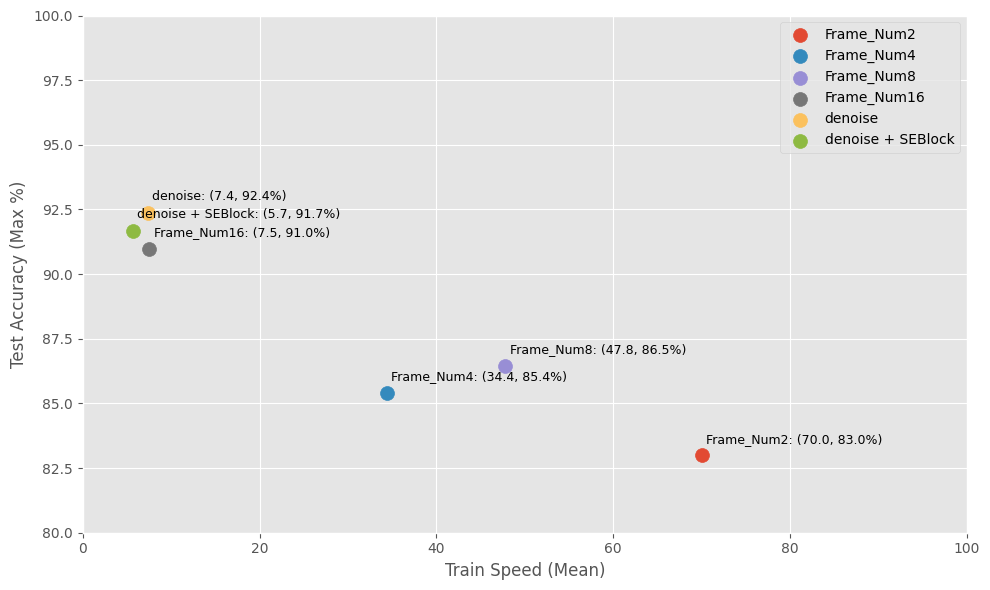
\includegraphics[width=0.45\textwidth]{figure/acc_speed.png}
    \caption{Speed-Accuracy Plot of All Training Processes}
    \label{fig:acc_speed_all}
\end{figure}
The Fig\ref{fig:acc_speed_all} illustrates the performance of the model under various training conditions during the experimental testing. The x-axis represents the average training speed, while the y-axis denotes the maximum accuracy achieved on the test set during the training process. Each point corresponds to a specific training scenario.

Among these, \texttt{Frame\_Num16} represents the baseline scenario, where the original dataset is divided into 16 frames for training the base model. In this case, the average training speed is 7.5, and the maximum accuracy on the test set is 91.0\%. The other points labeled with different frame numbers correspond to scenarios where the base dataset is divided into varying numbers of frames for training. It can be observed that as the number of frames decreases, the average training speed increases, but the test accuracy shows a decline.

The point labeled \texttt{denoise} represents the scenario where the base dataset is denoised before training the base model. Here, the training performance is the most optimal, with an average speed of 7.4—close to the baseline—and a prediction accuracy of 92.4\%, which is overall superior to the baseline. On the other hand, the point labeled \texttt{denoise + SEBlock} corresponds to the scenario where the denoised dataset is used to train the base model integrated with the SEBlock attention mechanism. While the accuracy in this case is also higher than the baseline, the average training speed significantly decreases to 5.7.

In summary, the results demonstrate that denoising the dataset leads to the most favorable training outcomes, achieving both competitive training speed and improved accuracy. However, integrating the SEBlock attention mechanism, although enhancing accuracy, incurs a notable reduction in training efficiency.

These findings highlight the importance of carefully balancing model complexity, data quality, and computational efficiency. While attention mechanisms like SEBlock offer theoretical benefits, their practical effectiveness depends on task-specific design and rigorous validation. Future work should focus on optimizing attention mechanisms for specific tasks, exploring dynamic approaches to reduce computational overhead, and further investigating the role of data preprocessing in improving model performance.

\section{Conclusion}
In this study, we explored the impact of spatio-temporal polarity coherent filtering and the integration of the SEBlock attention mechanism on model performance for gesture recognition using the DVS Gesture dataset. Our experiments systematically evaluated the effects of varying frame counts, denoising, and attention mechanisms on training efficiency and model accuracy, providing valuable insights into the trade-offs between computational complexity and predictive performance.

First, we demonstrated that the number of frames per event significantly influences model training speed and accuracy. While reducing the number of frames accelerates training, it also leads to information loss and reduced accuracy. The optimal balance was achieved with 16 frames, yielding the highest accuracy of 91.0\%, albeit at the slowest training speed of 7.5. Conversely, using only 2 frames resulted in the lowest accuracy of 83.0\% but increased training speed nearly tenfold.

Second, we showed that denoising the dataset using spatio-temporal polarity coherent filtering enhances model generalization. The denoised dataset consistently outperformed the original dataset in testing metrics, achieving a peak accuracy of 92.4\% compared to 91.0\% on the original dataset. Additionally, the denoised dataset maintained approximately 0.002 lower test loss and 1.4\% higher accuracy, underscoring the importance of data preprocessing in optimizing model performance.

Third, we investigated the integration of the SEBlock attention mechanism into the baseline model. While the attention-augmented model achieved higher accuracy than the baseline, its training speed was significantly slower (average speed: 5.7 vs. 7.4) due to increased computational overhead. Moreover, the attention mechanism introduced additional complexity without commensurate improvements in generalization, as evidenced by the consistently higher test loss (approximately 0.0014) and lower accuracy (0.7\% decrease) compared to the baseline.

These findings highlight the importance of carefully balancing model complexity, data quality, and computational efficiency. While attention mechanisms like SEBlock offer theoretical benefits, their practical effectiveness depends on task-specific design and rigorous validation. Future work should focus on optimizing attention mechanisms for specific tasks, exploring dynamic approaches to reduce computational overhead, and further investigating the role of data preprocessing in improving model performance.

In conclusion, our study underscores the critical role of data preprocessing and task-aware architecture design in enhancing model performance. By systematically evaluating the trade-offs between frame counts, denoising, and attention mechanisms, we provide a foundation for future research in optimizing gesture recognition models and other event-based vision tasks.
% \subsection{Abbreviations and Acronyms}\label{AA}
% Define abbreviations and acronyms the first time they are used in the text, 
% even after they have been defined in the abstract. Abbreviations such as 
% IEEE, SI, MKS, CGS, ac, dc, and rms do not have to be defined. Do not use 
% abbreviations in the title or heads unless they are unavoidable.

% \subsection{Units}
% \begin{itemize}
% \item Use either SI (MKS) or CGS as primary units. (SI units are encouraged.) English units may be used as secondary units (in parentheses). An exception would be the use of English units as identifiers in trade, such as ``3.5-inch disk drive''.
% \item Avoid combining SI and CGS units, such as current in amperes and magnetic field in oersteds. This often leads to confusion because equations do not balance dimensionally. If you must use mixed units, clearly state the units for each quantity that you use in an equation.
% \item Do not mix complete spellings and abbreviations of units: ``Wb/m\textsuperscript{2}'' or ``webers per square meter'', not ``webers/m\textsuperscript{2}''. Spell out units when they appear in text: ``. . . a few henries'', not ``. . . a few H''.
% \item Use a zero before decimal points: ``0.25'', not ``.25''. Use ``cm\textsuperscript{3}'', not ``cc''.)
% \end{itemize}

% \subsection{Equations}
% Number equations consecutively. To make your 
% equations more compact, you may use the solidus (~/~), the exp function, or 
% appropriate exponents. Italicize Roman symbols for quantities and variables, 
% but not Greek symbols. Use a long dash rather than a hyphen for a minus 
% sign. Punctuate equations with commas or periods when they are part of a 
% sentence, as in:
% \begin{equation}
% a+b=\gamma\label{eq}
% \end{equation}

% Be sure that the 
% symbols in your equation have been defined before or immediately following 
% the equation. Use ``\eqref{eq}'', not ``Eq.~\eqref{eq}'' or ``equation \eqref{eq}'', except at 
% the beginning of a sentence: ``Equation \eqref{eq} is . . .''

% \subsection{\LaTeX-Specific Advice}

% Please use ``soft'' (e.g., \verb|\eqref{Eq}|) cross references instead
% of ``hard'' references (e.g., \verb|(1)|). That will make it possible
% to combine sections, add equations, or change the order of figures or
% citations without having to go through the file line by line.

% Please don't use the \verb|{eqnarray}| equation environment. Use
% \verb|{align}| or \verb|{IEEEeqnarray}| instead. The \verb|{eqnarray}|
% environment leaves unsightly spaces around relation symbols.

% Please note that the \verb|{subequations}| environment in {\LaTeX}
% will increment the main equation counter even when there are no
% equation numbers displayed. If you forget that, you might write an
% article in which the equation numbers skip from (17) to (20), causing
% the copy editors to wonder if you've discovered a new method of
% counting.

% {\BibTeX} does not work by magic. It doesn't get the bibliographic
% data from thin air but from .bib files. If you use {\BibTeX} to produce a
% bibliography you must send the .bib files. 

% {\LaTeX} can't read your mind. If you assign the same label to a
% subsubsection and a table, you might find that Table I has been cross
% referenced as Table IV-B3. 

% {\LaTeX} does not have precognitive abilities. If you put a
% \verb|\label| command before the command that updates the counter it's
% supposed to be using, the label will pick up the last counter to be
% cross referenced instead. In particular, a \verb|\label| command
% should not go before the caption of a figure or a table.

% Do not use \verb|\nonumber| inside the \verb|{array}| environment. It
% will not stop equation numbers inside \verb|{array}| (there won't be
% any anyway) and it might stop a wanted equation number in the
% surrounding equation.

% \subsection{Some Common Mistakes}\label{SCM}
% \begin{itemize}
% \item The word ``data'' is plural, not singular.
% \item The subscript for the permeability of vacuum $\mu_{0}$, and other common scientific constants, is zero with subscript formatting, not a lowercase letter ``o''.
% \item In American English, commas, semicolons, periods, question and exclamation marks are located within quotation marks only when a complete thought or name is cited, such as a title or full quotation. When quotation marks are used, instead of a bold or italic typeface, to highlight a word or phrase, punctuation should appear outside of the quotation marks. A parenthetical phrase or statement at the end of a sentence is punctuated outside of the closing parenthesis (like this). (A parenthetical sentence is punctuated within the parentheses.)
% \item A graph within a graph is an ``inset'', not an ``insert''. The word alternatively is preferred to the word ``alternately'' (unless you really mean something that alternates).
% \item Do not use the word ``essentially'' to mean ``approximately'' or ``effectively''.
% \item In your paper title, if the words ``that uses'' can accurately replace the word ``using'', capitalize the ``u''; if not, keep using lower-cased.
% \item Be aware of the different meanings of the homophones ``affect'' and ``effect'', ``complement'' and ``compliment'', ``discreet'' and ``discrete'', ``principal'' and ``principle''.
% \item Do not confuse ``imply'' and ``infer''.
% \item The prefix ``non'' is not a word; it should be joined to the word it modifies, usually without a hyphen.
% \item There is no period after the ``et'' in the Latin abbreviation ``et al.''.
% \item The abbreviation ``i.e.'' means ``that is'', and the abbreviation ``e.g.'' means ``for example''.
% \end{itemize}
% An excellent style manual for science writers is \cite{b7}.

% \subsection{Authors and Affiliations}
% \textbf{The class file is designed for, but not limited to, six authors.} A 
% minimum of one author is required for all conference articles. Author names 
% should be listed starting from left to right and then moving down to the 
% next line. This is the author sequence that will be used in future citations 
% and by indexing services. Names should not be listed in columns nor group by 
% affiliation. Please keep your affiliations as succinct as possible (for 
% example, do not differentiate among departments of the same organization).

% \subsection{Identify the Headings}
% Headings, or heads, are organizational devices that guide the reader through 
% your paper. There are two types: component heads and text heads.

% Component heads identify the different components of your paper and are not 
% topically subordinate to each other. Examples include Acknowledgments and 
% References and, for these, the correct style to use is ``Heading 5''. Use 
% ``figure caption'' for your Figure captions, and ``table head'' for your 
% table title. Run-in heads, such as ``Abstract'', will require you to apply a 
% style (in this case, italic) in addition to the style provided by the drop 
% down menu to differentiate the head from the text.

% Text heads organize the topics on a relational, hierarchical basis. For 
% example, the paper title is the primary text head because all subsequent 
% material relates and elaborates on this one topic. If there are two or more 
% sub-topics, the next level head (uppercase Roman numerals) should be used 
% and, conversely, if there are not at least two sub-topics, then no subheads 
% should be introduced.

% \subsection{Figures and Tables}
% \paragraph{Positioning Figures and Tables} Place figures and tables at the top and 
% bottom of columns. Avoid placing them in the middle of columns. Large 
% figures and tables may span across both columns. Figure captions should be 
% below the figures; table heads should appear above the tables. Insert 
% figures and tables after they are cited in the text. Use the abbreviation 
% ``Fig.~\ref{fig}'', even at the beginning of a sentence.

% \begin{table}[htbp]
% \caption{Table Type Styles}
% \begin{center}
% \begin{tabular}{|c|c|c|c|}
% \hline
% \textbf{Table}&\multicolumn{3}{|c|}{\textbf{Table Column Head}} \\
% \cline{2-4} 
% \textbf{Head} & \textbf{\textit{Table column subhead}}& \textbf{\textit{Subhead}}& \textbf{\textit{Subhead}} \\
% \hline
% copy& More table copy$^{\mathrm{a}}$& &  \\
% \hline
% \multicolumn{4}{l}{$^{\mathrm{a}}$Sample of a Table footnote.}
% \end{tabular}
% \label{tab1}
% \end{center}
% \end{table}

% \begin{figure}[htbp]
% \centerline{
\includegraphics{figure/fig1.png}}
% \caption{Example of a figure caption.}
% \label{fig}
% \end{figure}

% Figure Labels: Use 8 point Times New Roman for Figure labels. Use words 
% rather than symbols or abbreviations when writing Figure axis labels to 
% avoid confusing the reader. As an example, write the quantity 
% ``Magnetization'', or ``Magnetization, M'', not just ``M''. If including 
% units in the label, present them within parentheses. Do not label axes only 
% with units. In the example, write ``Magnetization (A/m)'' or ``Magnetization 
% \{A[m(1)]\}'', not just ``A/m''. Do not label axes with a ratio of 
% quantities and units. For example, write ``Temperature (K)'', not 
% ``Temperature/K''.

% \section*{Acknowledgment}

% The preferred spelling of the word ``acknowledgment'' in America is without 
% an ``e'' after the ``g''. Avoid the stilted expression ``one of us (R. B. 
% G.) thanks $\ldots$''. Instead, try ``R. B. G. thanks$\ldots$''. Put sponsor 
% acknowledgments in the unnumbered footnote on the first page.

\section*{References}

% Please number citations consecutively within brackets \cite{b1}. The 
% sentence punctuation follows the bracket \cite{b2}. Refer simply to the reference 
% number, as in \cite{b3}---do not use ``Ref. \cite{b3}'' or ``reference \cite{b3}'' except at 
% the beginning of a sentence: ``Reference \cite{b3} was the first $\ldots$''

% Number footnotes separately in superscripts. Place the actual footnote at 
% the bottom of the column in which it was cited. Do not put footnotes in the 
% abstract or reference list. Use letters for table footnotes.

% Unless there are six authors or more give all authors' names; do not use 
% ``et al.''. Papers that have not been published, even if they have been 
% submitted for publication, should be cited as ``unpublished'' \cite{b4}. Papers 
% that have been accepted for publication should be cited as ``in press'' \cite{b5}. 
% Capitalize only the first word in a paper title, except for proper nouns and 
% element symbols.

% For papers published in translation journals, please give the English 
% citation first, followed by the original foreign-language citation \cite{b6}.

\bibliographystyle{IEEEtran}
\bibliography{reference}
% \vspace{12pt}
% \color{red}
% IEEE conference templates contain guidance text for composing and formatting conference papers. Please ensure that all template text is removed from your conference paper prior to submission to the conference. Failure to remove the template text from your paper may result in your paper not being published.

\end{document}
